\section{Wave Propagation}
\subsection{Radio Link Above an Idealized Ground Plane}
\subsubsection{Friis Transmission Formula}
\begin{tikzpicture}[>=Stealth]
    %% Idealized Ground
    \draw (0,0) -- (6.5, 0);
    \foreach \x in {0, .2, ..., 6.4}
        \draw[xshift=\x cm] (0, -.1) -- (.1, 0);
    %% Transmitter and Receiver
    \begin{scope}[xshift=.5cm, yshift=1.5cm]
        \draw node[] at (.5,.5){Tx};
        \draw (0,0) rectangle (1,1);
        \draw[->] (-.5, .5)node[above]{$P_{t0}$} -- (0, .5);
    \end{scope}
    \begin{scope}[xshift=5cm, yshift=1cm]
        \draw node[] at (.5,.5){Rx};
        \draw (0,0) rectangle (1,1);
        \draw[->] (1, .5) -- (1.5, .5)node[above]{$P_{r,\mathrm{max}}$};
    \end{scope}
    %% Contributions
    \draw[->, dotted] (1.5, 2) -- (5, 1.55);
    \draw[->, dotted] (1.5, 2) -- (3.45, 0) -- (5, 1.5);
    \draw[dashed] (1.5, 2) -- (1.5, -2) -- (3.45, 0);
    \fill[black!] (1.5, -2) circle (3pt) node[below]{image source};
    \fill[black!] (3.45, 0) circle (3pt) node[below right]{reflection point};
    %% Measurements
    \draw[{Bar}{Stealth}-{Stealth}{Bar}, thick] (1.7, 2) --node[right]{$h_t$} (1.7, 0);
    \draw[{Bar}{Stealth}-{Stealth}{Bar}, thick] (4.7, 1.5) --node[left]{$h_r$} (4.7, 0);
\end{tikzpicture}

\begin{align*}
    &P_{r,\mathrm{max}} =
    \begin{cases}
        P_{t0}\dfrac{G_1 G_2 \lambda^2}{4\pi^2r^2}, &R=+1\\
        P_{t0}\dfrac{G_1 G_2 (h_t h_r)^2}{r^4}, &R=-1
    \end{cases}\\
    &L_p = -10 \log_{10}\dfrac{P_{r,\mathrm{max}}}{P_t0}\text{ (pathloss)}\\
    &R =
    \begin{cases}
        +1, \quad \text{cond. grd., vert. pol., } f \ll \SI{30}{MHz},\\
        -1, \quad \text{dielec. ground, } f\geq \SI{30}{MHz}
    \end{cases}\\
    &\implies\text{VHF (and above) experience double pathloss!!!}
\end{align*}
\subsubsection{Fresnel Reflection and Transmission}
\begin{tikzpicture}
    %% Coordinates and material domains
    \filldraw[gray!30] (-3, -1.8) rectangle (3, 0);
    \draw[-{Stealth}] (-3,0) -- (3,0) node[right]{$x$};
    \draw[{Stealth}-{Stealth}] (0,-2) node[below]{$z$} -- (0, 2) node[above]{$\hat{n}$};
    %% Incident, Reflected and Transmitted Rays
    \draw[-{Stealth[length=3mm, width=2mm]}] (-2, 2) -- (0, 0);
    \draw[-{Stealth[length=3mm, width=2mm]}] (0 , 0) --node[below]{$R$} (1.8, 1.8);
    \draw[-{Stealth[length=3mm, width=2mm]}] (0 , 0) --node[right]{$T$} (1, -1.8);
    %% Angles
    \draw[red, {Stealth}-{Stealth}] (0, 1.2) arc (90:135:1.2cm);
    \draw node[red] at (-.3, .7){$\alpha_h$};
    \draw[orange, {Stealth}-{Stealth}] (0, 1.2) arc (90:45:1.2cm);
    \draw node[orange] at (.3, .7){$\alpha_r$};
    \draw[blue, {Stealth}-{Stealth}] (0, -1.4) arc (270:300:1.4cm);
    \draw node[blue] at (.3, -1){$\alpha_D$};
    %% Labels
    \draw node[draw] at (3, 1.8){$Z_1=\sqrt{\dfrac{\mu_1}{\epsilon_1}},\;k_1$};
    \draw node[draw, fill=white!] at (3, -1.8){$Z_2=\sqrt{\dfrac{\mu_2}{\epsilon_2}},\;k_2$};
    \draw node[] at (-2, .5){$\alpha_h = \alpha_r$};
    \draw node[] at (-1.5, -.6){$k_1 \sin\alpha_h = k_2 \sin\alpha_D$};
\end{tikzpicture}

\begin{enumerate}
    \itemsep0pt
    \item $\vec{E}$ $\parallel$ incidence plane (p-polarized)
        \begin{align*}
            &R_\parallel = \dfrac{E_r}{E_h} = \dfrac{H_r}{H_h} = \dfrac{Z_2\cos\alpha_D - Z_1\cos\alpha_h}{Z_1\cos\alpha_h + Z_2\cos\alpha_D},\\
            &T_{H\parallel} = \dfrac{H_D}{H_h} = \dfrac{2Z_1\cos\alpha_h}{Z_1\cos\alpha_h + Z_2\cos\alpha_D},\\
            &T_{E\parallel} = \dfrac{E_D}{E_h} = \dfrac{Z_2}{Z_1} T_{H\parallel}
        \end{align*}
    \item $\vec{E}$ $\perp$ incidence plane (s-polarized)
        \begin{align*}
            &R_\perp = \dfrac{E_r}{E_h} = \dfrac{H_r}{H_h} = \dfrac{Z_2\cos\alpha_h - Z_1\cos\alpha_D}{Z_1\cos\alpha_h + Z_2\cos\alpha_D},\\
            &T_{E\perp} = \dfrac{E_D}{E_h} = \dfrac{2Z_2\cos\alpha_h}{Z_1\cos\alpha_h + Z_2\cos\alpha_D},\\
            &T_{H\perp} = \dfrac{H_D}{H_h} = \dfrac{Z_1}{Z_2} T_{E\perp}
        \end{align*}
\end{enumerate}
\subsection{Wave Propagation in the Atmosphere}
\begin{itemize}
    \itemsep0pt
    \item $\epsilon_r$ \textit{decreases} with altitude (air density)
    \item The ray paths bend into the denser medium, i.e. \textit{towards the ground}
    \item \textbf{4/3-Earth} approximation corrects for atmospheric refraction; $R_E \to \dfrac{4}{3}R_E$
    \item 3-\SI{30}{MHz} short-wave frequencies:
        \begin{itemize}
            \itemsep0pt
            \item \textbf{Ground wave:} wave contributions propagating close to/along the ground
            \item \textbf{Sky wave:} wave contributions with one or more reflexions at the ionosphere
        \end{itemize}
    \item International Telecommunications Union (ITU) offers recommendations for correct modelling
\end{itemize}
\subsection{Terrestrial Wave Propagation Models}
Urban pathloss accord to the Hata model:
\begin{align*}
    L_p = &69.55 + 26.16\log_{10}f - 13.38\log_{10}h_t - a(h_r)\\
          &+ (44.9 - 6.55\log_{10}h_t)\log_{10}d
\end{align*}
Kuhlmann-Eibert Model for Pathloss:
\begin{align*}
    L_{\mathrm{med}} = &69.55 + 26.16\log_{10}(f/\si{MHz}) + A_d\\
                       &+ A_{\mathrm{dif}} + A_{\mathrm{lu}} + A_t + A_r + G_t + G_r
\end{align*}
\begin{tabular}{>{\(}l<{\)}p{5cm}}
    f: & frequency\\
    A_d: & pathloss due to distance along path profile\\
    A_{\mathrm{dif}}: & pathloss due to diffraction\\
    A_{\mathrm{lu}}: & pathloss due to land usage\\
    A_t: & pathloss due to height of transmitter antenna\\
    A_r: & pathloss due to height of receiver antenna\\
    G_t: & gain of transmitter antenna\\
    G_r: & gain of receiver antenna
\end{tabular}

\subsection{Geometrical Optics, Ray Techniques}
\begin{itemize}
    \itemsep0pt
    \item \textbf{Assumption:} far-field, locally plane wave (TEM), conservation of energy/phase along ray
    \item Several geometric ray solutions:
    \begin{align*}
        &\text{Plane Wave:}\\
        &E = E_1\,e^{-j\beta(r-r_1)}, &S = \mathrm{const.},\\
        &\text{Cylindrical Wave:}\\
        &E = E_1 \sqrt{\dfrac{r_1}{r}} e^{-j\beta_0(r - r_1)}, &S = \dfrac{r_1}{r}S_1,\\
        &\text{Spherical Wave:}\\
        &E = E_1 \dfrac{r_1}{r} e^{-j\beta_0(r - r_1)}, &S = \dfrac{r_1^2}{r^2}S_1
    \end{align*}
    \item \textbf{Astigmatic Ray} as general ray solution (1st term of Luneberg-Kline-series)
        \begin{align*}
            &\vec{E}(s) = \vec{E}(0) \sqrt{\dfrac{\rho_1\rho_2}{(\rho_1 + s)(\rho_2 + s)}} e^{-jks},\\
            &\rho_1,\rho_2\text{: define the caustics}
        \end{align*}
        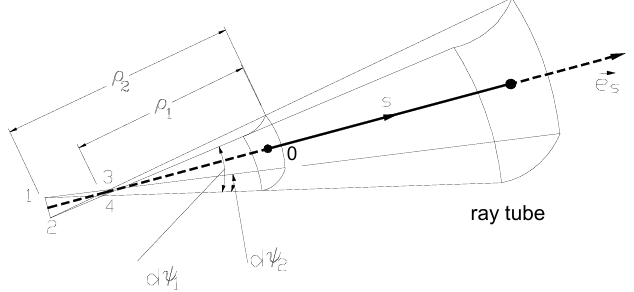
\includegraphics[width=.3\paperheight]{content/aawp/pictures/astigmatic_ray.png}
        \todo{Reflection of Astigmatic Ray}
\end{itemize}

\subsection{Geometrical Theory of Diffraction (GTD), Ray Techniques}
\subsubsection{Illustration of Reflection and Diffraction Phenomena}
    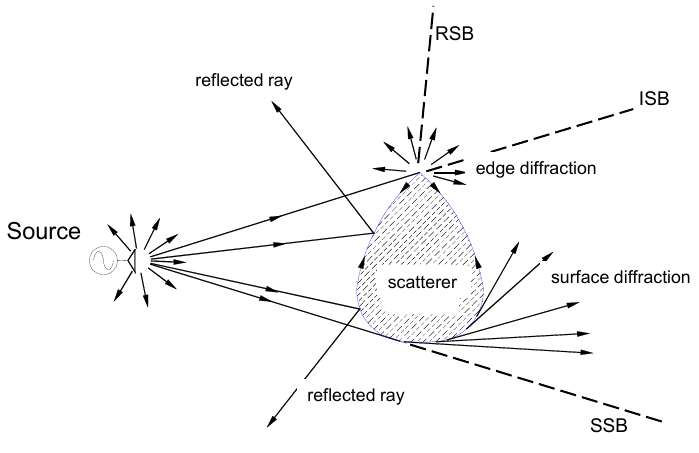
\includegraphics[width=.3\paperheight]{content/aawp/pictures/scatterer.png}
\subsubsection{Wedge Diffraction}
\begin{itemize}
    \itemsep0pt
    \item Infinite number of rays on a \textit{diffraction cone} (Keller cone).
        \fbox{%
            \parbox{6.5cm}{%
                \begin{align*}
                    &\vec{E}_k^d = \dyade{D} \cdot \vec{E}^{\mathrm{inc}} A(s)\,e^{-jks},\\
                    &A(s) = \sqrt{\dfrac{1}{s}}, \quad \text{\parbox{2cm}{(plane, cyl., conical wave onto straight edge)}}
                \end{align*}
                }}
            \item \textbf{Geometric Theory of Diffraction} (GTD) according to Keller, for points far away from shadow boundaries:\\
                \begin{tikzpicture}[
        >=Stealth
    ]
    \draw node(O)[] at (0, 0){};
    % Wedge
    \filldraw[draw=black!, fill=black!20] (O) -- (3,0) -- (3, -2) -- cycle;
    \fill (O) circle (2.5pt);
    % Rays
    \draw[->, thick] (2,2)node[right]{incident ray $\vec{r}^\prime$} -- (O);
    \draw[->, thick] (O) --node[below right]{$|\vec{r}| = s$} (-2,-1)node[below]{diffracted ray $\vec{r}$};
    % Angles
    \draw[<->] (2,0) arc (0:-33.5:2);
    \draw  (3.1,-.7)node[fill=black!10]{WA$= (2-n)\pi$};
    \draw[->] (1,0) arc (0:206.5:1);
    \draw (-1,.3)node[fill=white!]{$\varphi$};
    \draw[->] (1.5,0) arc (0:45:1.5);
    \draw (1.8, .55)node[fill=white!]{$\varphi^\prime = \beta_0$};
    % Legend
    \draw (-1.75, 2)node[]{$\parallel$: planar inc. ray};
    \draw (-1.8, 1.5)node[]{$\perp$: perp. inc. ray};
\end{tikzpicture}

                \begin{align*}
                    &D^{\parallel,\perp} = \dfrac{e^{j\pi/4} \sin(\pi/n)}{n\sqrt{2\pi k}\sin\beta_0}
                    \left[\dfrac{1}{\zeta(\varphi-\varphi^\prime)} \mp  \dfrac{1}{\zeta(\varphi+\varphi^\prime)}\right],\\
                    &\zeta(\Theta) = \cos\dfrac{\pi}{n} - \cos \dfrac{\Theta}{n}
                \end{align*}
    \item Opening angle of cone with respect to edge $\theta_d$ equal to angle of incident ray with respect to edge $\theta_i$.
\end{itemize}
\begin{center}
    \begin{equation*}
        \theta_i = \theta_d = \beta_0
    \end{equation*}
    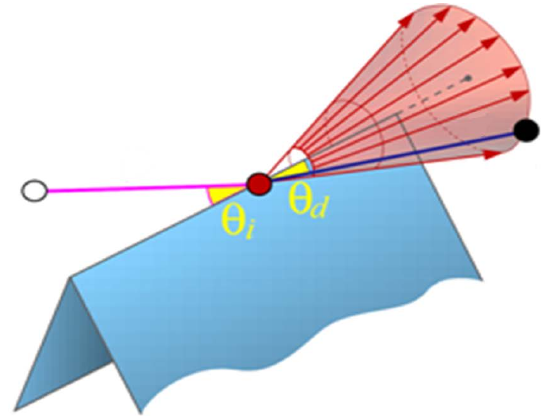
\includegraphics[width=4.5cm]{content/aawp/pictures/keller_cone.png}
\end{center}
\subsubsection{Ray Methods for Complex Environments}
\begin{itemize}
    \itemsep0pt
    \item \textbf{Deterministic Ray Tracing:} Exact ray path is determined for a given pair of transmitter and receiver locations.
    \item \textbf{Ray Launching:} Many rays are launched in arbitrary directions. Rays passing a receiver location in a certain distance are deleted.
\end{itemize}
